% =============================================================================
% Figure 1: Architecture comparison — Offline Sys-ID vs Online Real-to-Sim
% For ReSECT ICRA 2026 paper
%
% Compile standalone:
%   pdflatex fig_architecture_comparison.tex
%
% Or include in main paper:
%   \input{figs/fig_architecture_comparison.tex}
% =============================================================================
\documentclass[border=8pt]{standalone}

\usepackage{tikz}
\usepackage{amsmath, amssymb}
\usepackage{xcolor}

\usetikzlibrary{
  arrows.meta,
  positioning,
  shapes.geometric,
  fit,
  backgrounds,
  calc,
  decorations.pathreplacing,
}

% ---- Color palette (muted, professional) ----
\definecolor{realcolor}{RGB}{200,60,60}        % real phantom (red)
\definecolor{simcolor}{RGB}{50,110,180}        % simulator (blue)
\definecolor{losscolor}{RGB}{125,80,160}       % loss (purple)
\definecolor{gradcolor}{RGB}{50,130,80}        % gradient (green)
\definecolor{adamcolor}{RGB}{90,90,90}         % optimizer (gray)
\definecolor{histcolor}{RGB}{210,170,50}       % history buffer (amber)
\definecolor{outputcolor}{RGB}{40,40,40}       % output (dark gray)
\definecolor{bgleft}{RGB}{248,242,240}         % before bg (warm tone)
\definecolor{bgright}{RGB}{240,245,250}        % after bg (cool tone)

% ---- Node styles ----
\tikzset{
  realnode/.style={
    rectangle, rounded corners=2pt, draw=realcolor, very thick,
    fill=realcolor!8, minimum width=2.4cm, minimum height=0.75cm,
    font=\small, align=center, text=realcolor!50!black
  },
  simnode/.style={
    rectangle, rounded corners=2pt, draw=simcolor, very thick,
    fill=simcolor!8, minimum width=2.4cm, minimum height=0.75cm,
    font=\small, align=center, text=simcolor!50!black
  },
  lossnode/.style={
    ellipse, draw=losscolor, very thick, fill=losscolor!10,
    minimum width=2.8cm, minimum height=0.7cm,
    font=\small, align=center, text=losscolor!40!black
  },
  gradnode/.style={
    rectangle, draw=gradcolor, very thick, fill=gradcolor!10,
    minimum width=2.8cm, minimum height=0.7cm,
    font=\small, align=center, text=gradcolor!40!black
  },
  adamnode/.style={
    rectangle, rounded corners=2pt, draw=adamcolor, very thick,
    fill=adamcolor!8, minimum width=2.4cm, minimum height=0.7cm,
    font=\small, align=center, text=adamcolor!30!black
  },
  histnode/.style={
    rectangle, draw=histcolor, very thick, fill=histcolor!12,
    rounded corners=3pt,
    minimum width=2.4cm, minimum height=0.6cm,
    font=\footnotesize, align=center, text=histcolor!30!black
  },
  outputnode/.style={
    rectangle, draw=outputcolor, very thick, fill=outputcolor!10,
    minimum width=2.4cm, minimum height=0.7cm,
    font=\small, align=center, text=outputcolor
  },
  loopcontainer/.style={
    rectangle, dashed, thick, rounded corners=8pt,
    inner sep=12pt, draw=black!50,
  },
  innerloopcontainer/.style={
    rectangle, dotted, thick, rounded corners=6pt,
    inner sep=8pt, draw=gradcolor!70,
  },
  flow/.style={
    -{Latex[length=2.5mm, width=2mm]}, thick,
  },
  dataflow/.style={
    flow, draw=black!70,
  },
  gradflow/.style={
    flow, draw=gradcolor, line width=1.2pt,
  },
  realflow/.style={
    flow, draw=realcolor!80,
  },
  simflow/.style={
    flow, draw=simcolor!80,
  },
  feedback/.style={
    flow, dashed, draw=histcolor!70!black, line width=1pt,
  },
  panellabel/.style={
    font=\bfseries\large, align=center,
  },
}

\begin{document}

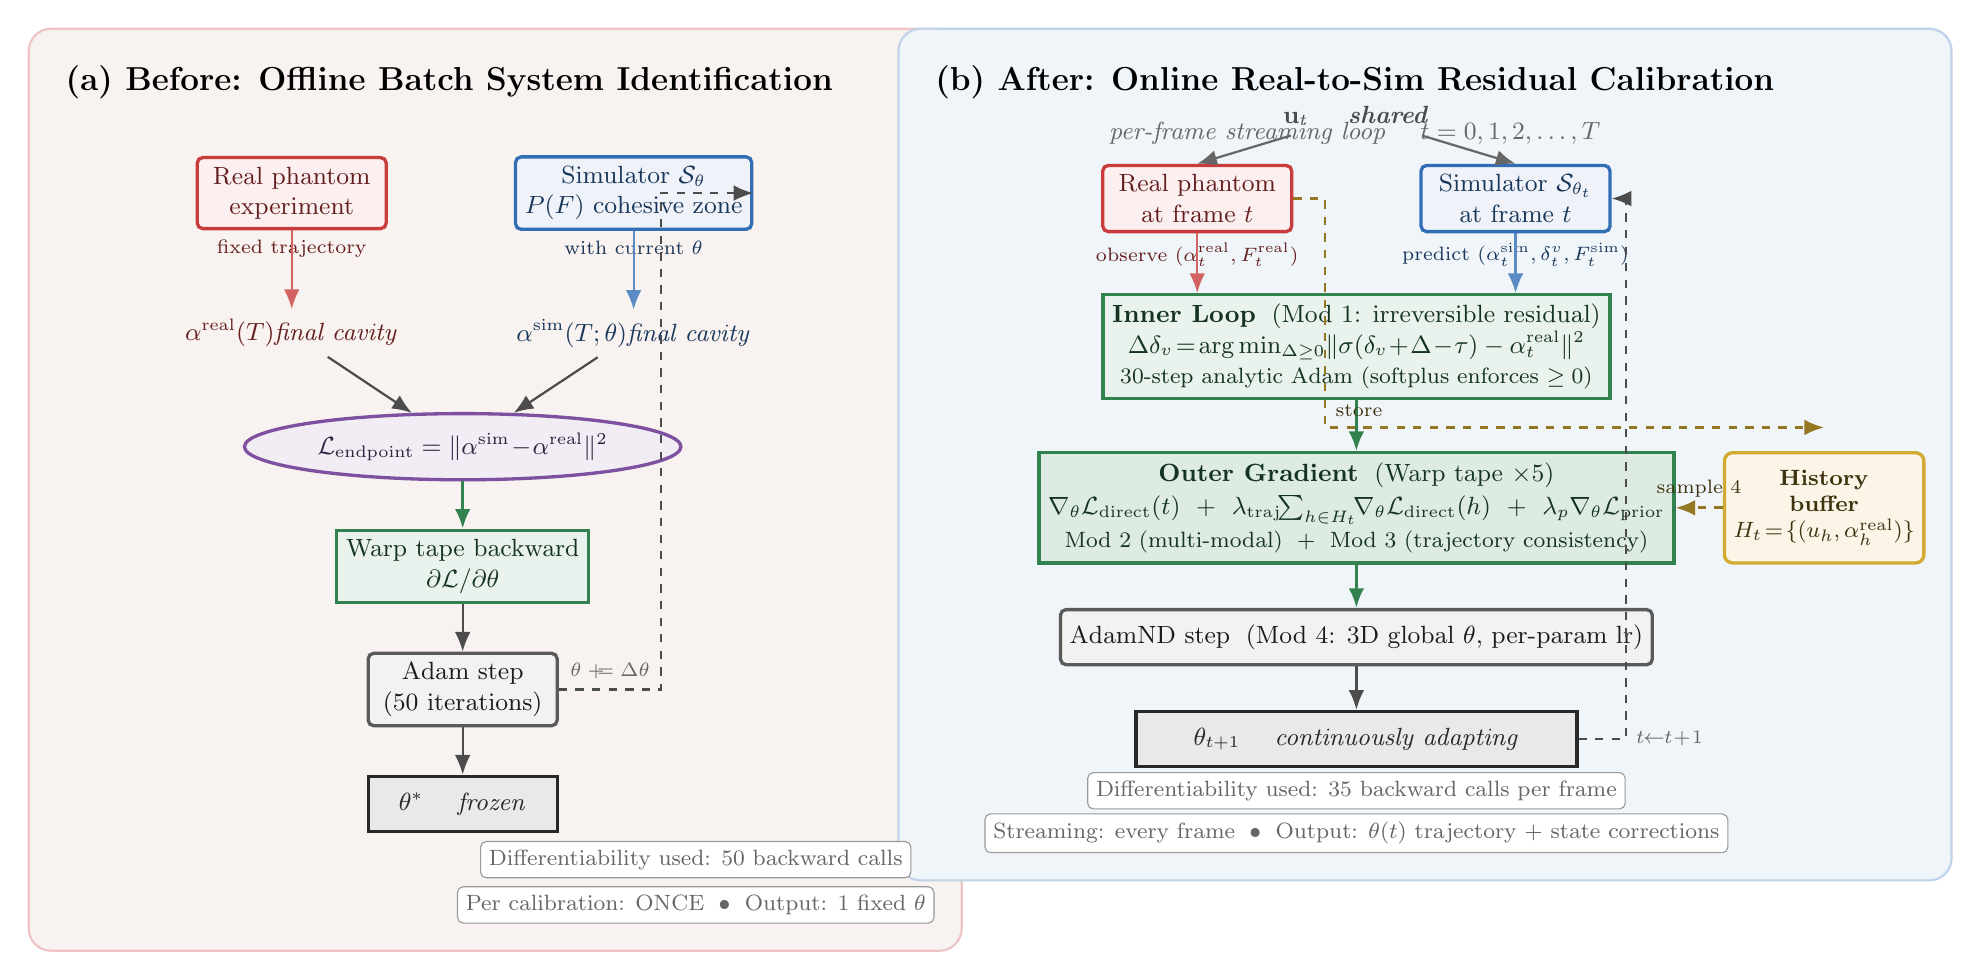
\begin{tikzpicture}[node distance=0.7cm and 0.9cm]

% =============================================================================
% (a) BEFORE — Offline Batch Sys-ID  (LEFT PANEL)
% =============================================================================

\begin{scope}[local bounding box=panelA]

  % Title
  \node[panellabel] (titleA)
    {(a) Before: Offline Batch System Identification};

  % Real phantom node (top-left)
  \node[realnode, below=0.6cm of titleA, xshift=-2.0cm]
    (realA) {Real phantom\\experiment};
  \node[font=\scriptsize, below=0pt of realA, text=realcolor!50!black]
    {fixed trajectory};

  % Simulator node (top-right)
  \node[simnode, right=1.6cm of realA]
    (simA) {Simulator $\mathcal{S}_\theta$\\$P(F)$ cohesive zone};
  \node[font=\scriptsize, below=0pt of simA, text=simcolor!50!black]
    {with current $\theta$};

  % Final cavities (data nodes)
  \node[font=\small, below=1.0cm of realA, text=realcolor!50!black]
    (alphaR) {$\alpha^{\text{real}}(T)$\\\textit{final cavity}};
  \node[font=\small, below=1.0cm of simA, text=simcolor!50!black]
    (alphaS) {$\alpha^{\text{sim}}(T;\theta)$\\\textit{final cavity}};

  % Loss node
  \node[lossnode, below=1.0cm of $(alphaR)!0.5!(alphaS)$]
    (lossA) {$\mathcal{L}_{\text{endpoint}} = \|\alpha^{\text{sim}}\!-\!\alpha^{\text{real}}\|^2$};

  % Gradient node
  \node[gradnode, below=0.6cm of lossA]
    (gradA) {Warp tape backward\\$\partial \mathcal{L} / \partial \theta$};

  % Adam node
  \node[adamnode, below=0.6cm of gradA]
    (adamA) {Adam step\\(50 iterations)};

  % Output theta (frozen)
  \node[outputnode, below=0.6cm of adamA]
    (outA) {$\theta^*$ \quad \textit{frozen}};

  % Arrows — top to bottom
  \draw[realflow] (realA) -- (alphaR);
  \draw[simflow]  (simA)  -- (alphaS);
  \draw[dataflow] (alphaR) -- (lossA);
  \draw[dataflow] (alphaS) -- (lossA);
  \draw[gradflow] (lossA) -- (gradA);
  \draw[dataflow] (gradA) -- (adamA);
  \draw[dataflow] (adamA) -- (outA);

  % Adam loop (back-arrow showing iteration)
  \draw[dataflow, dashed]
    (adamA.east) -- ++(1.3, 0)
    node[font=\scriptsize, midway, above, text=black!60]{$\theta \mathrel{+}\!\!= \Delta\theta$}
    |- (simA.east);

  % Annotation: "ONCE per calibration"
  \node[font=\footnotesize, draw=black!40, fill=white, rounded corners=2pt,
        inner sep=3pt, below right=0.1cm and -1.0cm of outA, text=black!60]
    (annA1) {Differentiability used: 50 backward calls};
  \node[font=\footnotesize, draw=black!40, fill=white, rounded corners=2pt,
        inner sep=3pt, below=0.1cm of annA1, text=black!60]
    {Per calibration: ONCE  $\;\bullet\;$  Output: 1 fixed $\theta$};

\end{scope}

% =============================================================================
% (b) AFTER — Online Real-to-Sim Streaming  (RIGHT PANEL)
% =============================================================================

\begin{scope}[local bounding box=panelB, shift={(11.5cm, 0)}]

  % Title
  \node[panellabel] (titleB)
    {(b) After: Online Real-to-Sim Residual Calibration};

  \node[font=\small\itshape, below=0.05cm of titleB, text=black!60]
    {per-frame streaming loop \quad $t = 0, 1, 2, \ldots, T$};

  % Real and Sim (now PER FRAME)
  \node[realnode, below=0.7cm of titleB, xshift=-2.0cm]
    (realB) {Real phantom\\at frame $t$};
  \node[font=\scriptsize, below=0pt of realB, text=realcolor!50!black]
    {observe $(\alpha^{\text{real}}_t, F^{\text{real}}_t)$};

  \node[simnode, right=1.6cm of realB]
    (simB) {Simulator $\mathcal{S}_{\theta_t}$\\at frame $t$};
  \node[font=\scriptsize, below=0pt of simB, text=simcolor!50!black]
    {predict $(\alpha^{\text{sim}}_t, \delta^v_t, F^{\text{sim}}_t)$};

  % Shared control u_t (above, between)
  \node[font=\small\bfseries, above=0.8cm of $(realB)!0.5!(simB)$, text=black!70]
    (controlB) {$\mathbf{u}_t$ \quad \textit{shared}};
  \draw[flow, draw=black!60] (controlB) -- (realB.north);
  \draw[flow, draw=black!60] (controlB) -- (simB.north);

  % Inner loop block
  \node[gradnode, below=1.2cm of $(realB)!0.5!(simB)$,
        minimum width=5.6cm, minimum height=1.15cm]
    (innerB) {\textbf{Inner Loop} \;(Mod 1: irreversible residual)\\
              $\Delta\delta_v \!=\! \arg\min_{\Delta \geq 0}\!
                \|\sigma(\delta_v\!+\!\Delta\!-\!\tau) - \alpha^{\text{real}}_t\|^2$\\
              \footnotesize 30-step analytic Adam (softplus enforces $\geq 0$)};

  % Outer gradient block (3 channels)
  \node[gradnode, below=0.65cm of innerB,
        minimum width=5.6cm, minimum height=1.4cm,
        fill=gradcolor!16]
    (outerB) {\textbf{Outer Gradient} \;(Warp tape $\times 5$)\\[1pt]
              $\nabla_\theta \mathcal{L}_{\text{direct}}(t)$ \;+\;
              $\lambda_{\text{traj}} \!\!\sum_{h \in H_t}\!\! \nabla_\theta \mathcal{L}_{\text{direct}}(h)$ \;+\;
              $\lambda_p \nabla_\theta \mathcal{L}_{\text{prior}}$\\[1pt]
              \footnotesize Mod 2 (multi-modal) \;+\; Mod 3 (trajectory consistency)};

  % AdamND step
  \node[adamnode, below=0.55cm of outerB,
        minimum width=5.6cm, minimum height=0.7cm]
    (adamB) {AdamND step \;(Mod 4: 3D global $\theta$, per-param lr)};

  % Theta_t output (streaming)
  \node[outputnode, below=0.55cm of adamB,
        minimum width=5.6cm, minimum height=0.7cm]
    (outB) {$\theta_{t+1}$ \quad \textit{continuously adapting}};

  % History buffer
  \node[histnode, right=0.6cm of outerB,
        minimum width=2.5cm, minimum height=1.4cm, align=center]
    (histB) {\textbf{History}\\\textbf{buffer}\\$H_t \!=\! \{(u_h, \alpha^{\text{real}}_h)\}$};

  % Data flow within panel B
  \draw[realflow] (realB) -- (innerB.north -| realB);
  \draw[simflow]  (simB)  -- (innerB.north -| simB);
  \draw[gradflow] (innerB) -- (outerB);
  \draw[gradflow] (outerB) -- (adamB);
  \draw[dataflow] (adamB) -- (outB);

  % L_traj sampling from history (dashed, amber)
  \draw[feedback] (histB.west) -- (outerB.east)
    node[font=\scriptsize, midway, above, text=histcolor!30!black,
         sloped]{sample 4};

  % New frame storage to history
  \draw[feedback] (realB.east) -| ++(0.4,0) |- ($(histB.north) + (0,0.3)$)
    node[font=\scriptsize, midway, above right, text=histcolor!30!black]
    {store};

  % Feedback theta_t to sim (next frame)
  \draw[dataflow, dashed]
    (outB.east) -- ++(0.6, 0)
    node[font=\scriptsize, right, text=black!60]
    {$t \!\!\leftarrow\!\! t\!+\!1$}
    |- (simB.east);

  % Annotations
  \node[font=\footnotesize, draw=black!40, fill=white, rounded corners=2pt,
        inner sep=3pt, below=0.05cm of outB, text=black!60]
    (annB1) {Differentiability used: 35 backward calls per frame};
  \node[font=\footnotesize, draw=black!40, fill=white, rounded corners=2pt,
        inner sep=3pt, below=0.05cm of annB1, text=black!60]
    {Streaming: every frame  $\;\bullet\;$  Output: $\theta(t)$ trajectory + state corrections};

\end{scope}

% =============================================================================
% Backgrounds — slight tinting to separate panels
% =============================================================================
\begin{scope}[on background layer]
  \node[fit=(panelA), inner sep=10pt,
        fill=bgleft, rounded corners=8pt, draw=realcolor!30, thick] {};
  \node[fit=(panelB), inner sep=10pt,
        fill=bgright, rounded corners=8pt, draw=simcolor!30, thick] {};
\end{scope}

% =============================================================================
% Vertical separator (optional visual divider)
% =============================================================================
%\draw[dashed, black!20, line width=0.8pt]
%  ($(panelA.north east)!0.5!(panelB.north west) - (0,-0.5)$) --
%  ($(panelA.south east)!0.5!(panelB.south west) - (0,0.5)$);

\end{tikzpicture}

\end{document}
